% !TeX root = ../main.tex

% DOCX body[24]
\section{Method}\label{sec:method}

% DOCX body[25]
\subsection{Problem Definition}\label{sec:problem-definition}

% DOCX body[26]
In zero-shot learning, classes are divided into two disjoint sets: seen classes and unseen classes. The model is trained only on samples from seen classes, while unseen classes appear only at test time. As a result, it cannot directly learn the data distributions of unseen classes and must instead use class-level semantic information to transfer audio-visual knowledge learned from seen classes. In the more demanding generalized zero-shot setting, test samples come from the union of seen and unseen classes. The model must generalize to unseen classes, retain discrimination among seen classes, and overcome prediction bias toward seen classes. This setting is therefore considered more representative of practical applications. AVGZSL addresses this problem by jointly using the visual and audio content of videos. Although actions and sound events can corroborate one another, their associations with class semantics vary across samples, making seen-to-unseen transfer more challenging. Formally, let ${\mathcal{C}}_{s}$ and ${\mathcal{C}}_{u}$ denote the sets of seen and unseen classes, respectively, with ${\mathcal{C}}_{s}\cap {\mathcal{C}}_{u}=\emptyset .$ The training set contains audio-visual samples from seen classes and is denoted by $\mathcal{S}=\{({x}_{n}^{v},{x}_{n}^{a},{y}_{n}){\}}_{n=1}^{N},$ where ${x}_{n}^{v}$ and ${x}_{n}^{a}$ are the visual and audio streams of training video $n,$ ${y}_{n}\in {\mathcal{C}}_{s}$ is its ground-truth label, and $N$ is the number of training samples. The objective is to learn a decision function $h:({x}^{v},{x}^{a})\mapsto {\mathcal{C}}_{s}\cup {\mathcal{C}}_{u}$ that correctly classifies test samples from the union of seen and unseen classes.

% DOCX body[27]
\subsection{Overall Architecture}\label{sec:overall-architecture}

% DOCX body[28]
Most existing AVGZSL methods use class label embeddings for classification in the final matching stage, separating video encoding from class semantics. In contrast, our framework uses discriminatively optimized class embeddings as conditioning signals throughout encoding to guide temporal grounding, interaction, and fusion for both modalities, as illustrated in Fig.~\ref{fig:architecture}. The framework comprises three components: DSPO, CGTA, and DMIF. First, DSPO expands class names into fine-grained descriptions, constructs initial class embeddings, and improves class separability while preserving semantic structure. This component addresses insufficient discrimination in pre-trained text embeddings and ambiguous boundaries between similar classes, providing reliable semantic references for subsequent temporal aggregation and alignment. Second, CGTA introduces the optimized class semantics into visual and audio sequence encoding and uses continuous Gaussian distributions to localize and aggregate class-relevant segments, preventing irrelevant segments from diluting key evidence. Finally, DMIF organizes the selected audio-visual evidence through separate intra-modal and inter-modal relationships and adaptively adjusts their fusion weights to mitigate the interference and modality bias associated with direct concatenation.

% DOCX body[29]
% DOCX body[29]
\begin{figure*}[pos=t]
\centering
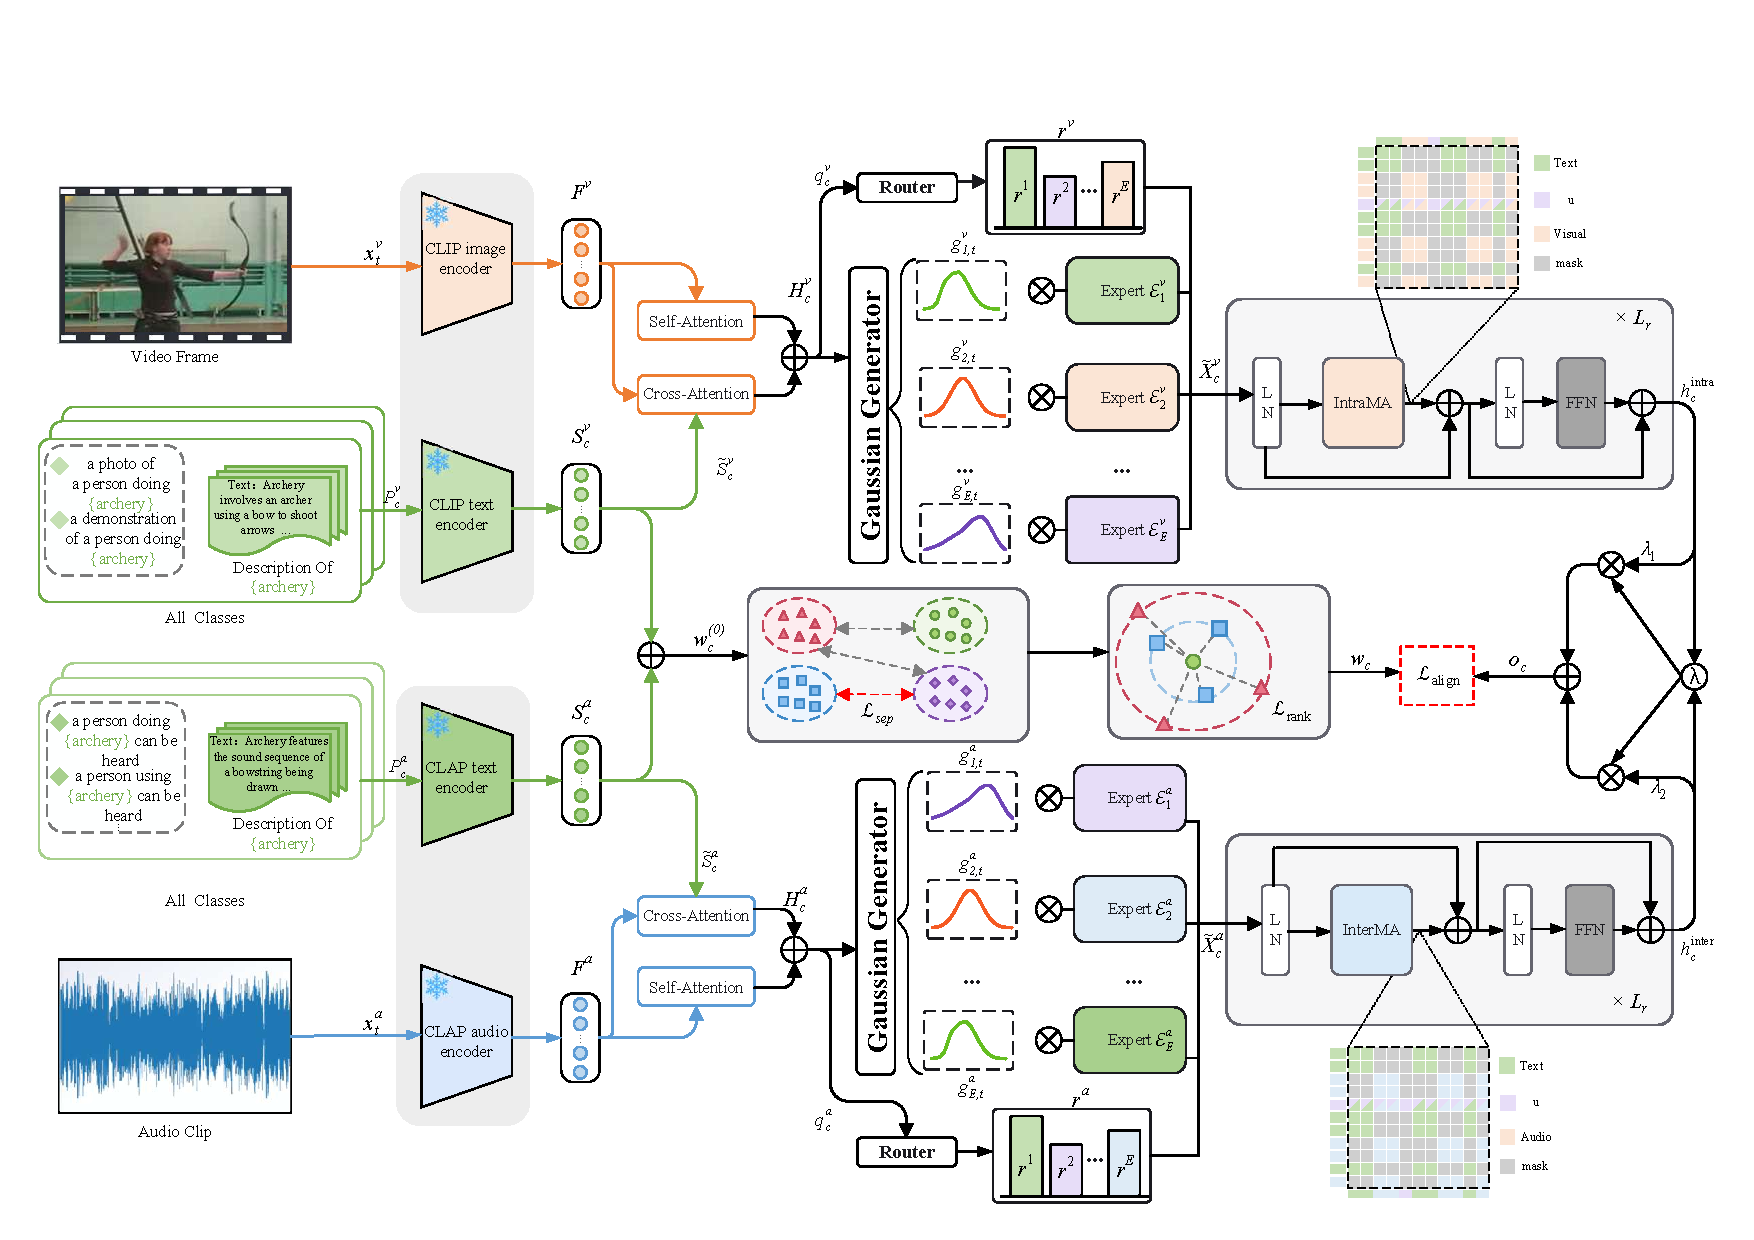
\includegraphics[pagebox=mediabox,width=\textwidth,trim={12bp 11bp 13bp 51bp},clip]{figures/SGTG.pdf}
\caption{Overall architecture of SGTG. An input video is divided into temporally aligned consecutive segments, from which frozen CLIP image and CLAP audio encoders extract visual and audio sequences. In parallel, frozen text encoders transform the candidate class\textquoteright{}s visual and auditory descriptions into description embeddings, and DSPO produces optimized class embeddings that are subsequently fixed. CGTA conditions each modality sequence on its description embeddings and uses the class embedding to query independent visual and audio Gaussian experts with adaptive routing. Continuous weighting and aggregation produce enhanced sequences and direct audio-visual evidence. DMIF then models temporal relationships through intra-modal and inter-modal encoder branches and applies a three-way dynamic Softmax gate conditioned on the direct evidence and candidate class. Finally, a projection network maps the fused representation to a class-conditioned embedding.}
\label{fig:architecture}
\end{figure*}


% DOCX body[31]
\subsection{Discriminative Semantic Prototype Optimization}\label{sec:discriminative-semantic-prototype-optimization}

% DOCX body[32]
Class label embeddings bridge seen and unseen classes in AVGZSL. Embeddings from pre-trained models such as CLIP and CLAP preserve useful semantic relationships. For example, \textquotedblleft{}playing guitar\textquotedblright{} is closer to \textquotedblleft{}playing violin\textquotedblright{} than to \textquotedblleft{}dog barking\textquotedblright{} in semantic space, and such relationships underpin zero-shot transfer. However, these embeddings are not optimized for the target classification task. Class embeddings of semantically similar classes can be too close to distinguish similar actions or sounds. Conversely, maximizing class separability alone tends to push all class embeddings toward an equidistant configuration, erasing the distinction between semantically related and unrelated classes and disrupting the semantic relationships required for transfer. To resolve this conflict, we develop Discriminative Semantic Prototype Optimization (DSPO) based on class embedding optimization \cite{mo2024easy}. Starting from the original text embeddings, DSPO learns class embeddings with improved separability while retaining their semantic relationships. Specifically, it first constructs text embeddings of class descriptions and then jointly optimizes the class embeddings under two competing objectives: class separability and semantic preservation.

% DOCX body[33]
For class $c,$ let ${\mathcal{P}}_{c}^{v}$ and ${\mathcal{P}}_{c}^{a}$ denote its sets of visual and auditory descriptions, respectively, each containing $P$ descriptions. We pass the two sets through the pre-trained CLIP and CLAP text encoders and stack their outputs row-wise to obtain two matrices of description embeddings, with one encoded description per row:

% DOCX body[34]
% DOCX body[34]; M015
\begin{equation}
\label{eq:visual-description-encoding}
{S}_{c}^{v}={\Phi }_{\mathrm{T}}^{v}\left( {\mathcal{P}}_{c}^{v}\right) \in {\mathbb{R}}^{P\times {d}_{t}^{v}}
\end{equation}


% DOCX body[35]
% DOCX body[35]; M016
\begin{equation}
\label{eq:audio-description-encoding}
{S}_{c}^{a}={\Phi }_{\mathrm{T}}^{a}\left( {\mathcal{P}}_{c}^{a}\right) \in {\mathbb{R}}^{P\times {d}_{t}^{a}}
\end{equation}

% DOCX body[36]
\noindent\unskip where ${\Phi }_{\mathrm{T}}^{v}(\cdot )$ and ${\Phi }_{\mathrm{T}}^{a}(\cdot )$ denote the frozen CLIP and CLAP text encoders, respectively, and ${d}_{t}^{v}$ and ${d}_{t}^{a}$ are their text-embedding dimensions. At the class level, we apply ${\ell }_{2}$ normalization to each row of ${S}_{c}^{v}$ and ${S}_{c}^{a}$ and average the normalized rows to obtain the modality-specific class label embeddings ${\overline{s}}_{c}^{v}\in {\mathbb{R}}^{{d}_{t}^{v}}$ and ${\overline{s}}_{c}^{a}\in {\mathbb{R}}^{{d}_{t}^{a}}.$ Concatenating and normalizing these embeddings gives the initial class embedding:

% DOCX body[37]
% DOCX body[37]; M026
\begin{equation}
\label{eq:initial-class-embedding}
{w}_{c}^{(0)}=\frac{\left[ {\overline{s}}_{c}^{v}\Vert {\overline{s}}_{c}^{a}\right] }{{\left\Vert \left[ {\overline{s}}_{c}^{v}\Vert {\overline{s}}_{c}^{a}\right] \right\Vert }_{2}}\in {\mathbb{R}}^{{d}_{s}}
\end{equation}

% DOCX body[38]
\noindent\unskip where $[\cdot \Vert \cdot ]$ denotes vector concatenation, and ${d}_{s}={d}_{t}^{v}+{d}_{t}^{a}$ is the dimensionality of the class embedding space. Row-wise normalization preserves the directional meaning of the averaged vectors, while global normalization places all class embeddings on the unit sphere, allowing class relationships to be characterized by Euclidean distance.

% DOCX body[39]
Starting from these initial class embeddings, we optimize a new set of class embeddings $\{{w}_{c}{\}}_{c\in \mathcal{C}},$ where $\mathcal{C}={\mathcal{C}}_{s}\cup {\mathcal{C}}_{u},$ subject to ${\left\Vert {w}_{c}\right\Vert }_{2}=1.$ To enhance class separability, we maximize the distance from each class embedding to its nearest neighbor by minimizing the following class-separation loss:

% DOCX body[40]
% DOCX body[40]; M032
\begin{equation}
\label{eq:separation-loss}
{\mathcal{L}}_{sep}=-\sum _{c\in \mathcal{C}}\underset{{c}^{\prime }\in \mathcal{C},{c}^{\prime }\ne c}{\mathrm{min}}{\left\Vert {w}_{c}-{w}_{{c}^{\prime }}\right\Vert }_{2}
\end{equation}

% DOCX body[41]
\noindent\unskip where the inner $\mathrm{min}$ selects the closest other class embedding to class $c,$ and the outer summation accumulates the loss over all classes. Because the loss acts only on each class\textquoteright{}s nearest neighbor, it prioritizes separation of the most easily confused class pairs. We further introduce a margin ranking loss for semantic preservation that maintains the relative order of distances between the initial class embeddings. For distinct classes $c,i\in\mathcal{C}$, let $d_{ci}^{(0)}=\lVert w_c^{(0)}-w_i^{(0)}\rVert_2$ and $d_{ci}=\lVert w_c-w_i\rVert_2$ denote the initial and optimized distances, respectively. For pairwise distinct $c,i,j\in\mathcal{C}$, define $\eta_{cij}=\operatorname{sign}(d_{ci}^{(0)}-d_{cj}^{(0)})$, and let $\mathcal{T}$ contain all such ordered triplets. The margin ranking loss is then

% DOCX body[42]
% DOCX body[42]; M035. Equivalent notation; distances/sign defined in body[41].
\begingroup\postdisplaypenalty=10000
\begin{equation}
\label{eq:ranking-loss}
\mathcal{L}_{rank}=\sum_{(c,i,j)\in\mathcal{T}}\max\bigl\{0,\Delta-\eta_{cij}(d_{ci}-d_{cj})\bigr\}.
\end{equation}
\endgroup

% DOCX body[43]
\noindent\unskip where $\Delta >0$ is the margin coefficient, and $sign(\cdot )$ is the sign function. The triple summation in \eqref{eq:ranking-loss} scales cubically with the number of classes. For a large class set, it can be approximated by randomly sampling a fixed number of triplets at each update. We jointly optimize the two objectives using a trade-off coefficient:

% DOCX body[44]
% DOCX body[44]; M038
\begin{equation}
\label{eq:prototype-objective}
\mathcal{L}=\underset{\{{w}_{c}{\}}_{c\in \mathcal{C}},{\left\Vert {w}_{c}\right\Vert }_{2}=1}{\mathrm{min}}(1-\alpha ){\mathcal{L}}_{rank}+\alpha {\mathcal{L}}_{sep}
\end{equation}

% DOCX body[45]
\noindent\unskip where $\alpha \in (0,1)$ balances class separability against semantic preservation. We initialize the class embeddings with ${w}_{c}={w}_{c}^{(0)},$ solve \eqref{eq:prototype-objective} by gradient descent, and renormalize each class embedding onto the unit sphere after every update. Once optimization converges, all class embeddings $\{{w}_{c}\}$ are fixed. The optimized class embeddings serve not only as alignment targets for classification in Section~\ref{sec:joint-embedding-training-and-inference} but also as conditional queries in the next module, guiding the model to actively localize evidence relevant to each candidate class in long audio-visual sequences.

% DOCX body[46]
\subsection{Class-Conditioned Gaussian Temporal Aggregation}\label{sec:class-conditioned-gaussian-temporal-aggregation}

% DOCX body[47]
Not every segment of a long video is relevant to its class. In a \textquotedblleft{}wood thrush calling\textquotedblright{} video, for example, the critical bird call may occupy only a small portion of the audio, with environmental noise dominating the remaining duration. Likewise, the decisive action in \textquotedblleft{}basketball dunk\textquotedblright{} occurs only within a short frame interval. Under the conventional class-agnostic global encoding paradigm, uniform pooling dilutes such local evidence with redundant segments. For an unseen class without training samples, class semantics are particularly important for actively searching potentially relevant temporal regions. To address this problem, we propose Class-Conditioned Gaussian Temporal Aggregation (CGTA), which uses optimized class embeddings as encoding conditions rather than only as matching references. It first injects description embeddings into the visual and audio sequences to condition their representations on the candidate class. It then generates multiple continuous Gaussian distributions to independently localize and aggregate class-relevant segments along the two modality timelines. CGTA adapts question-aware fusion and temporal integration of Gaussian experts \cite{kim2025qatiger} by replacing question features with description embeddings and optimized class embeddings.

% DOCX body[48]
\textbf{Class-semantic-aware early fusion. }We divide each input video into $T$ non-overlapping consecutive temporal segments. Segment $t$ contains a representative image ${x}_{t}^{v}$ and its corresponding audio waveform ${x}_{t}^{a}.$ Frozen pre-trained encoders extract the segment-level visual and audio features:

% DOCX body[49]
% DOCX body[49]; M046
\begin{equation}
\label{eq:visual-feature}
{F}_{t}^{v}={\Phi }_{\mathrm{V}}\left( {x}_{t}^{v}\right) \in {\mathbb{R}}^{{d}_{v}}
\end{equation}


% DOCX body[50]
% DOCX body[50]; M047
\begin{equation}
\label{eq:audio-feature}
{F}_{t}^{a}={\Phi }_{\mathrm{A}}\left( {x}_{t}^{a}\right) \in {\mathbb{R}}^{{d}_{a}}
\end{equation}

% DOCX body[51]
\noindent\unskip where ${\Phi }_{\mathrm{V}}(\cdot )$ and ${\Phi }_{\mathrm{A}}(\cdot )$ denote the CLIP image and CLAP audio encoders, respectively, while ${d}_{v}$ and ${d}_{a}$ are the corresponding feature dimensions. After stacking the segment features in temporal order to form ${F}^{v}\in {\mathbb{R}}^{T\times {d}_{v}}$ and ${F}^{a}\in {\mathbb{R}}^{T\times {d}_{a}},$ we map them into a shared $d$-dimensional space through two learnable linear projections and add temporal positional encodings:

% DOCX body[52]
% DOCX body[52]; M055
\begin{equation}
\label{eq:feature-projection}
V={F}^{v}{W}_{v}+PE,\quad \quad A={F}^{a}{W}_{a}+PE
\end{equation}

% DOCX body[53]
\noindent\unskip where ${W}_{v}\in {\mathbb{R}}^{{d}_{v}\times d}$ and ${W}_{a}\in {\mathbb{R}}^{{d}_{a}\times d}$ are projection matrices, and $PE\in {\mathbb{R}}^{T\times d}$ is a learnable temporal positional encoding. The two sequences share the same positional encodings to preserve segment order and maintain temporal alignment across modalities. For consistent notation, we define standard scaled dot-product attention as

% DOCX body[54]
% DOCX body[54]; M059
\begin{equation}
\label{eq:attention}
Attn(X,Y)=Softmax\left( \frac{X{W}_{Q}{\left( Y{W}_{K}\right) }^{\top }}{\sqrt{{d}_{k}}}\right) Y{W}_{V}
\end{equation}

% DOCX body[55]
\noindent\unskip where $X$ supplies the queries and $Y$ supplies both the keys and values, with ${W}_{Q},{W}_{K}\in {\mathbb{R}}^{d\times {d}_{k}}$ and ${W}_{V}\in {\mathbb{R}}^{d\times d}.$ The $\mathrm{Softmax}$ operation normalizes along the key dimension. We denote self-attention by $SA(X)=Attn(X,X)$ and cross-attention by $CA(X,Y)=Attn(X,Y).$

% DOCX body[56]
We then inject the description embeddings from Section~\ref{sec:discriminative-semantic-prototype-optimization} into the two modality sequences as keys and values. For candidate class $c,$ learnable projections first map the description embeddings to the shared dimensionality: ${\widetilde{S}}_{c}^{v}={S}_{c}^{v}{W}_{s}^{v}\in {\mathbb{R}}^{P\times d}$ and ${\widetilde{S}}_{c}^{a}={S}_{c}^{a}{W}_{s}^{a}\in {\mathbb{R}}^{P\times d},$ where ${W}_{s}^{v}\in {\mathbb{R}}^{{d}_{t}^{v}\times d}$ and ${W}_{s}^{a}\in {\mathbb{R}}^{{d}_{t}^{a}\times d}.$ The class-conditioned sequence encodings are defined as

% DOCX body[57]
% DOCX body[57]; M072
\begin{equation}
\label{eq:conditioned-visual}
{H}_{c}^{v}=V+SA(V)+CA\left( V,{\widetilde{S}}_{c}^{v}\right) 
\end{equation}


% DOCX body[58]
% DOCX body[58]; M073
\begin{equation}
\label{eq:conditioned-audio}
{H}_{c}^{a}=A+SA(A)+CA\left( A,{\widetilde{S}}_{c}^{a}\right) 
\end{equation}

% DOCX body[59]
\noindent\unskip where ${H}_{c}^{v},{H}_{c}^{a}\in {\mathbb{R}}^{T\times d}$ denote the visual and audio sequences conditioned on class $c,$ respectively.

% DOCX body[60]
\textbf{Temporal integration of Gaussian experts. }Given the class-conditioned sequences, we further localize and aggregate class-relevant evidence along the temporal axis. We use Gaussian distributions as soft masks in a Mixture of Experts (MoE) framework, with independent weighted aggregation for audio and visual features. First, the optimized class embedding queries each conditioned sequence to obtain an aggregated representation for each modality conditioned on the candidate class:

% DOCX body[61]
% DOCX body[61]; M076
\begin{equation}
\label{eq:class-queries}
{q}_{c}^{v}=CA\left( \psi ({w}_{c}),{H}_{c}^{v}\right) ,\quad \quad {q}_{c}^{a}=CA\left( \psi ({w}_{c}),{H}_{c}^{a}\right) 
\end{equation}

% DOCX body[62]
\noindent\unskip where $\psi ({w}_{c})={W}_{\psi }{w}_{c}+{b}_{\psi }\in {\mathbb{R}}^{d}$ is a learnable transformation from the ${d}_{s}$-dimensional class embedding space to the shared feature space. Since $\psi ({w}_{c})$ acts as a single-row attention query, the aggregated representations satisfy ${q}_{c}^{v},{q}_{c}^{a}\in {\mathbb{R}}^{d}.$ We then generate distribution parameters for $E$ Gaussian experts in each modality. Using $m\in \{v,a\}$ to index the modality, we define

% DOCX body[63]
% DOCX body[63]; M083
\begin{equation}
\label{eq:gaussian-parameters}
\left[ {\delta }^{m};{\varepsilon }^{m}\right] ={q}_{c}^{m}{W}_{g}^{m}
\end{equation}


% DOCX body[64]
% DOCX body[64]; M084
\begin{equation}
\label{eq:gaussian-centers-widths}
{\mu }_{k}^{m}=\frac{2k-1}{2E}+\frac{1}{2E}\mathrm{tanh}\left( {\delta }_{k}^{m}\right) ,\quad \quad {\sigma }_{k}^{m}=Softplus\left( {\varepsilon }_{k}^{m}\right) 
\end{equation}

% DOCX body[65]
\noindent\unskip where ${W}_{g}^{m}\in {\mathbb{R}}^{d\times 2E}$ is the parameter-generation matrix. Equation \eqref{eq:gaussian-parameters} divides the $2E$-dimensional output into two equal parts: center offsets ${\delta }^{m}\in {\mathbb{R}}^{E}$ and width parameters ${\varepsilon }^{m}\in {\mathbb{R}}^{E},$ where $k=1,\ldots ,E$ indexes the experts, while ${\mu }_{k}^{m}$ and ${\sigma }_{k}^{m}$ are the Gaussian center and standard deviation of expert $k$ on the normalized temporal axis $[0,1].$ The Gaussian soft mask of expert $k$ at time step $t$ and its temporally normalized form are given by

% DOCX body[66]
% DOCX body[66]; M096
\begin{equation}
\label{eq:gaussian-mask}
{g}_{k,t}^{m}=exp\left( -\frac{{\left( t/T-{\mu }_{k}^{m}\right) }^{2}}{2{\left( {\sigma }_{k}^{m}\right) }^{2}}\right) 
\end{equation}


% DOCX body[67]
% DOCX body[67]; M097
\begin{equation}
\label{eq:normalized-mask}
{\widehat{g}}_{k,t}^{m}=\frac{{g}_{k,t}^{m}}{\sum _{{t}^{\prime }=1}^{T}{g}_{k,{t}^{\prime }}^{m}}
\end{equation}

% DOCX body[68]
\noindent\unskip where the mask ${g}_{k,t}^{m}\in \left( 0,1\right] $ peaks at the expert center and decays continuously with temporal distance, while ${\widehat{g}}_{k,t}^{m}$ is normalized along time and sums to $1.$ To determine the contribution of each expert for the current sample and candidate class, a router generates routing values (expert weights) from the aggregated representation:

% DOCX body[69]
% DOCX body[69]; M101
\begin{equation}
\label{eq:expert-routing}
{r}^{m}=Softmax\left( {q}_{c}^{m}{W}_{r}^{m}\right) \in {\mathbb{R}}^{E}
\end{equation}

% DOCX body[70]
\noindent\unskip where ${W}_{r}^{m}\in {\mathbb{R}}^{d\times E}$ is the learnable router weight matrix, and $\mathrm{Softmax}$ normalizes along the expert dimension. The component ${r}_{k}^{m}$ indicates the importance of expert $k.$ Each expert is further equipped with a position-wise linear transformation ${\mathcal{E}}_{k}^{m}:{\mathbb{R}}^{d}\to {\mathbb{R}}^{d},$ and its outputs are integrated in two ways. First, we retain the temporal axis to obtain an enhanced sequence weighted by class relevance:

% DOCX body[71]
% DOCX body[71]; M107
\begin{equation}
\label{eq:enhanced-sequence}
{\widetilde{X}}_{c,t}^{m}=\sum _{k=1}^{E}{r}_{k}^{m}{g}_{k,t}^{m}{\mathcal{E}}_{k}^{m}\left( {H}_{c,t}^{m}\right) 
\end{equation}


% DOCX body[72]
Second, we aggregate along time to obtain a compact temporal evidence vector:

% DOCX body[73]
% DOCX body[73]; M108
\begin{equation}
\label{eq:direct-evidence}
{\widetilde{e}}_{c}^{m}=\sum _{k=1}^{E}{r}_{k}^{m}\sum _{t=1}^{T}{\widehat{g}}_{k,t}^{m}{\mathcal{E}}_{k}^{m}\left( {H}_{c,t}^{m}\right) 
\end{equation}

% DOCX body[74]
\noindent\unskip where ${H}_{c,t}^{m}\in {\mathbb{R}}^{d}$ is row $t$ of the conditioned sequence, with ${\widetilde{X}}_{c}^{m}\in {\mathbb{R}}^{T\times d}$ and ${\widetilde{e}}_{c}^{m}\in {\mathbb{R}}^{d}.$ Equation \eqref{eq:direct-evidence} directly summarizes evidence through Gaussian-weighted aggregation without passing through the subsequent masked attention branches. We fuse the temporally aggregated representations of the two modalities into a direct evidence representation:

% DOCX body[75]
% DOCX body[75]; M113
\begin{equation}
\label{eq:direct-av-evidence}
{\widetilde{e}}_{c}^{av}={W}_{e}\left[ {\widetilde{e}}_{c}^{v}\Vert {\widetilde{e}}_{c}^{a}\right] +{b}_{e}\in {\mathbb{R}}^{d}
\end{equation}

% DOCX body[76]
\noindent\unskip where ${W}_{e}\in {\mathbb{R}}^{2d\times d}$ and ${b}_{e}\in {\mathbb{R}}^{d}$ are learnable parameters. At this point, candidate-class guidance has produced two enhanced sequences that emphasize class-relevant segments and a robust direct evidence vector.

% DOCX body[77]
\subsection{Decoupled Modality Interaction and Gated Fusion}\label{sec:decoupled-modality-interaction-and-gated-fusion}

% DOCX body[78]
Audio and visual content are not always strongly correlated in real-world videos. Visual observations may contain occlusions or irrelevant actions, whereas audio may include background music and environmental noise. Modality dependence also varies across classes: instrument performances require corroboration between sound and movement, while the discriminative information for some classes comes almost entirely from one modality. If the two sequences are fused through indiscriminate global attention, cross-modal attention may propagate irrelevant content as context and cause modality interference. Conversely, a fixed preference for one modality may induce bias toward seen classes and undermine unseen-class generalization. To address these issues, we design Decoupled Modality Interaction and Gated Fusion (DMIF). Following Semi-IIN \cite{lin2025semiinn}, two complementary attention masks implement IntraMA and InterMA in independent branches, while a sample- and class-conditioned gate dynamically adjusts the contributions of intra-modal representations, inter-modal representations, and direct temporal evidence.

% DOCX body[79]
Specifically, we concatenate the two enhanced sequences with a learnable special token for feature aggregation to form the input to each branch. For branch $b\in \{intra,inter\},$

% DOCX body[80]
% DOCX body[80]; M117
\begin{equation}
\label{eq:branch-input}
{Z}_{c}^{(0),b}=\left[ {u}^{b};{\widetilde{X}}_{c}^{a};{\widetilde{X}}_{c}^{v}\right] \in {\mathbb{R}}^{(2T+1)\times d}
\end{equation}

% DOCX body[81]
\noindent\unskip where ${u}^{b}\in {\mathbb{R}}^{d}$ is a branch-specific learnable special token at position $0.$ Audio tokens occupy positions $1$ through $T,$ and visual tokens occupy positions $T+1$ through $2T.$ Let ${\Omega }_{a}=\{1,\ldots ,T\}$ and ${\Omega }_{v}=\{T+1,\ldots ,2T\}$ denote the audio and visual position sets, respectively. We define the two mask matrices ${M}^{\mathrm{intra}},{M}^{\mathrm{inter}}\in {\mathbb{R}}^{(2T+1)\times (2T+1)}$ as

% DOCX body[82]
% DOCX body[82]; M127
\begin{equation}
\label{eq:intra-mask}
{M}_{pq}^{\mathrm{intra}}=\left\{ \begin{array}{ll}0,&p=0,\text{ or }p,q\in {\Omega }_{a},\text{ or }p,q\in {\Omega }_{v}\\-\infty ,&\text{otherwise}\end{array}\right . 
\end{equation}


% DOCX body[83]
% DOCX body[83]; M128
\begin{equation}
\label{eq:inter-mask}
\begin{aligned} {M}_{pq}^{\mathrm{inter}}=\left\{\begin{array}{ll}0,&\begin{aligned}[t] &p=0,\text{ or }p\in {\Omega}_{a},q\in {\Omega}_{v},\\ &\text{ or }p\in {\Omega}_{v},q\in {\Omega}_{a}\end{aligned}\\-\infty,&\text{otherwise}\end{array}\right.\end{aligned}
\end{equation}

% DOCX body[84]
\noindent\unskip where $p$ is the query position and $q$ is the key position. Masked attention adds the mask matrix after the scaled dot product and before $\mathrm{Softmax}:$

% DOCX body[85]
% DOCX body[85]; M132
\begin{equation}
\label{eq:masked-attention}
MA(Z;M)=Softmax\left( \frac{Z{W}_{Q}{\left( Z{W}_{K}\right) }^{\top }}{\sqrt{{d}_{k}}}+M\right) Z{W}_{V}
\end{equation}

% DOCX body[86]
\noindent\unskip where entries set to $-\infty $ receive zero attention weight after $\mathrm{Softmax},$ thereby controlling which positions are visible. Each branch stacks ${L}_{r}$ masked attention units. At layer $l,$ the representation is updated as

% DOCX body[87]
% DOCX body[87]; M137
\begin{equation}
\label{eq:branch-updates}
\begin{gathered}{\widehat{Z}}_{c}^{(l),b}=MA\left( \mathrm{LN}\left( {Z}_{c}^{(l-1),b}\right) ;{M}^{b}\right) +{Z}_{c}^{(l-1),b},\\{Z}_{c}^{(l),b}=FFN\left( \mathrm{LN}\left( {\widehat{Z}}_{c}^{(l),b}\right) \right) +{\widehat{Z}}_{c}^{(l),b}\end{gathered}
\end{equation}

% DOCX body[88]
\noindent\unskip where $LN(\cdot )$ denotes layer normalization, $FFN(\cdot )$ is a two-layer feed-forward network with $\mathrm{ReLU}$ activation, and $l=1,\ldots ,{L}_{r}.$ After ${L}_{r}$ updates, the output at each branch\textquoteright{}s special-token position serves as its representation. Specifically, ${h}_{c}^{\mathrm{intra}}={Z}_{c}^{({L}_{r}),intra}[0]\in {\mathbb{R}}^{d}$ summarizes stable intra-modal cues after Gaussian weighting, whereas ${h}_{c}^{\mathrm{inter}}={Z}_{c}^{({L}_{r}),inter}[0]\in {\mathbb{R}}^{d}$ summarizes complementary corroborating information across the two modalities.

% DOCX body[89]
For candidate class $c,$ the model now has three evidence representations: the intra-modal representation ${h}_{c}^{\mathrm{intra}},$ the inter-modal representation ${h}_{c}^{\mathrm{inter}},$ and the direct temporal evidence ${\widetilde{e}}_{c}^{av}.$ We therefore construct a dynamic gate conditioned on these representations and the candidate-class embedding:

% DOCX body[90]
% DOCX body[90]; M149; two-line native-math layout, locally 9pt.
\begingroup\small\postdisplaypenalty=10000
\setlength{\jot}{2pt}
\begin{equation}
\label{eq:three-way-gate}
\begin{aligned}
\lambda={}&Softmax\bigl({W}_{2}\mathrm{ReLU}\bigl({W}_{1}\bigl[{h}_{c}^{\mathrm{intra}}\Vert {h}_{c}^{\mathrm{inter}}\\
&{}\quad\Vert{\widetilde{e}}_{c}^{av}\Vert\psi({w}_{c})\bigr]+{b}_{1}\bigr)+{b}_{2}\bigr)
\end{aligned}
\end{equation}
\endgroup


% DOCX body[91]
% DOCX body[91]; M150
\begin{equation}
\label{eq:gated-fusion}
{o}_{c}={\lambda }_{1}{h}_{c}^{\mathrm{intra}}+{\lambda }_{2}{h}_{c}^{\mathrm{inter}}+{\lambda }_{3}{\widetilde{e}}_{c}^{av}
\end{equation}

% DOCX body[92]
\noindent\unskip where ${W}_{1}\in {\mathbb{R}}^{4d\times d},$ ${W}_{2}\in {\mathbb{R}}^{d\times 3},$ ${b}_{1}\in {\mathbb{R}}^{d},$ and ${b}_{2}\in {\mathbb{R}}^{3}$ are learnable parameters. The $\mathrm{Softmax}$ operation normalizes across the three branches, so $\lambda =({\lambda }_{1},{\lambda }_{2},{\lambda }_{3})$ satisfies ${\lambda }_{1}+{\lambda }_{2}+{\lambda }_{3}=1.$ The vector ${o}_{c}\in {\mathbb{R}}^{d}$ is the fused representation for candidate class $c.$ It combines all evidence that has been selected, organized, and adaptively weighted.

% Balance the remaining two columns before the planned experiment pages.
% DOCX body[93]
\subsection{Joint Embedding, Training, and Inference}\label{sec:joint-embedding-training-and-inference}

% DOCX body[94]
A two-layer projection network maps the fused representation back into the ${d}_{s}$-dimensional semantic space of the class embeddings:

% DOCX body[95]
% DOCX body[95]; M161
\begin{equation}
\label{eq:semantic-projection}
{z}_{c}={W}_{z2}\mathrm{ReLU}\left( {W}_{z1}{o}_{c}+{b}_{z1}\right) +{b}_{z2}\in {\mathbb{R}}^{{d}_{s}}
\end{equation}

% DOCX body[96]
\noindent\unskip where ${W}_{z1}\in {\mathbb{R}}^{d\times d},$ ${W}_{z2}\in {\mathbb{R}}^{d\times {d}_{s}},$ ${b}_{z1}\in {\mathbb{R}}^{d},$ and ${b}_{z2}\in {\mathbb{R}}^{{d}_{s}}$ are learnable parameters. The similarity between sample $x=({x}^{v},{x}^{a})$ and candidate class $c$ is defined as temperature-scaled cosine similarity:

% DOCX body[97]
% DOCX body[97]; M168
\begin{equation}
\label{eq:similarity}
s(x,c)=\frac{{z}_{c}^{\top }{w}_{c}}{{\left\Vert {z}_{c}\right\Vert }_{2}\tau }
\end{equation}

% DOCX body[98]
\noindent\unskip where $\tau $ is the temperature parameter. Because class embedding ${w}_{c}$ already lies on the unit sphere, it requires no additional normalization. Based on this similarity function, training proceeds in two sequential optimization stages, and inference uses the same scoring rule. The two training objectives are described below.

% DOCX body[99]
\textbf{Class embedding optimization. }The first-stage objective is given in \eqref{eq:separation-loss}\textendash{}\eqref{eq:prototype-objective}. Starting from the initial class embeddings ${w}_{c}^{(0)},$ we optimize the class embeddings of all classes $\{{w}_{c}\}$ through gradient descent. This stage uses only class names and their textual descriptions; it neither updates network parameters nor uses audio-visual samples. Once convergence is reached, the class embeddings are fixed to provide discriminative, semantically structured conditional queries and alignment targets for the second stage.

% DOCX body[100]
\textbf{Supervised audio-visual language alignment. }In the second stage, we train the main network using a supervised text-audio-visual contrastive loss inspired by \cite{mo2024easy}. It pulls each training sample\textquoteright{}s class-conditioned embedding toward its ground-truth class embedding and pushes it away from the class embeddings of other seen classes:

% DOCX body[101]
% DOCX body[101]; M173
\begin{equation}
\label{eq:alignment-loss}
{\mathcal{L}}_{align}=-\frac{1}{N}\sum _{n=1}^{N}\mathrm{log}\frac{\mathrm{exp}\left( s\left( {x}_{n},{y}_{n}\right) \right) }{\sum _{c\in {\mathcal{C}}_{s}}\mathrm{exp}\left( s\left( {x}_{n},c\right) \right) }
\end{equation}

% DOCX body[102]
\noindent\unskip where ${x}_{n}=({x}_{n}^{v},{x}_{n}^{a})$ is training sample $n,$ and ${y}_{n}$ is its ground-truth label. The denominator normalizes over all seen classes ${\mathcal{C}}_{s}.$

% DOCX body[103]
At inference time, given a test sample $x,$ the model performs a conditioned forward pass for each candidate in ${\mathcal{C}}_{s}\cup {\mathcal{C}}_{u}$ and computes its similarity score. Because classification training uses only seen classes, the scores are biased toward these classes. We apply calibrated stacking \cite{chao2016gzsl} to penalize seen-class scores during inference:

% DOCX body[104]
% DOCX body[104]; M180
\begin{equation}
\label{eq:calibrated-inference}
\widehat{c}=\underset{c\in {\mathcal{C}}_{s}\cup {\mathcal{C}}_{u}}{\mathrm{argmax}}\left[ s(x,c)-\gamma \cdot \mathbb{1}\left( c\in {\mathcal{C}}_{s}\right) \right] 
\end{equation}

% DOCX body[105]
\noindent\unskip where $\mathbb{1}(\cdot )$ is the indicator function, and $\gamma \ge 0$ is the calibration coefficient. This coefficient affects only seen-class scores during inference and does not alter the training procedure.
